% Oguzhan Gencoglu
% LATEX Presentation template

\documentclass{beamer}

\usepackage{marvosym}
\usepackage[version=3]{mhchem}
\usepackage{amsmath}
\usepackage{epstopdf}
\usepackage{MnSymbol,wasysym}
\usepackage{color}
\usepackage{emerald}

\DeclareMathSizes{10}{10}{10}{10}

% You can uncomment the themes below if you would like to use a different
% one:
%\usetheme{AnnArbor}
%\usetheme{Antibes}
%\usetheme{Bergen}
%\usetheme{Berkeley}
%\usetheme{Berlin}
%\usetheme{Boadilla}
%\usetheme{boxes}
%\usetheme{CambridgeUS}
%\usetheme{Copenhagen}
%\usetheme{Darmstadt}
%\usetheme{default}
%\usetheme{Frankfurt}
%\usetheme{Goettingen}
%\usetheme{Hannover}
%\usetheme{Ilmenau}
%\usetheme{JuanLesPins}
\usetheme{Luebeck}
%\usetheme{Madrid}
%\usetheme{Malmoe}
%\usetheme{Marburg}
%\usetheme{Montpellier}
%\usetheme{PaloAlto}
%\usetheme{Pittsburgh}
%\usetheme{Rochester}
%\usetheme{Singapore}
%\usetheme{Szeged}
%\usetheme{Warsaw}

\title{Why is your data valuable? \\ A machine learning and AI perspective}

% A subtitle is optional and this may be deleted

\author{Oguzhan (Ouz) Gencoglu}
% - Give the names in the same order as the appear in the paper.
% - Use the \inst{?} command only if the authors have different
%   affiliation.

\institute[TUT] % (optional, but mostly needed)
{
  %
  Tampere University of Technology
}
% - Use the \inst command only if there are several affiliations.
% - Keep it simple, no one is interested in your street address.

\date{MyData2016 - 2 September 2016}
% - Either use conference name or its abbreviation.
% - Not really informative to the audience, more for people (including
%   yourself) who are reading the slides online

\subject{Machine Learning, Artificial Intelligence, Data Privacy, Personal Data}
% This is only inserted into the PDF information catalog. Can be left
% out. 

% If you have a file called "university-logo-filename.xxx", where xxx
% is a graphic format that can be processed by latex or pdflatex,
% resp., then you can add a logo as follows:

% \pgfdeclareimage[height=0.5cm]{university-logo}{university-logo-filename}
% \logo{\pgfuseimage{university-logo}}

% Delete this, if you do not want the table of contents to pop up at
% the beginning of each subsection:
\AtBeginSubsection[]
{
\begin{frame}<beamer>{Outline}
	\tableofcontents[currentsection,currentsubsection]
\end{frame}
}

% Let's get started
\begin{document}

\setbeamerfont{footnote}{size=\tiny}

\begin{frame}
	\titlepage
\end{frame}

\begin{frame}{Outline}
	\tableofcontents
	% You might wish to add the option [pausesections]
\end{frame}

% Section and subsections will appear in the presentation overview
% and table of contents.
\section{What Exactly Is Machine Learning?}
\subsection{Some Terminology}

\begin{frame}{Some Terminology}
		\begin{figure}
	  		\vspace*{0.1cm}
			\centering
			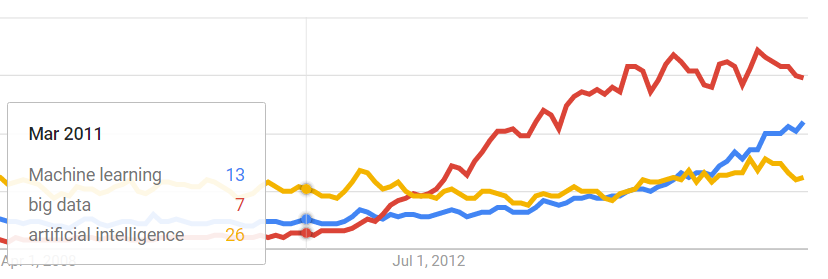
\includegraphics[trim = 0mm 0mm 0mm 0mm, clip, width=9.0cm]{gtrends.png}
			\label{fig:res4}
		\end{figure}
\end{frame}

\subsection{Recent Highlights}
\begin{frame}{Recent Highlights}
		\begin{figure}
	  		\vspace*{0.0cm}
			\centering
			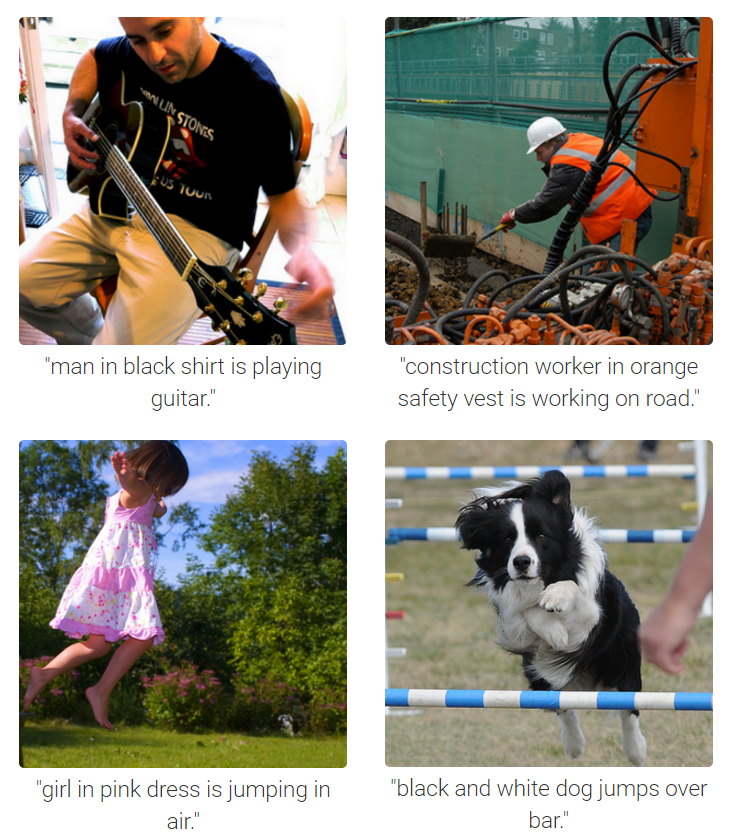
\includegraphics[trim = 0mm 0mm 0mm 0mm, clip, width=5.7cm]{visualdesc.PNG}
			\label{fig:res4}
		\end{figure}
\end{frame}

\begin{frame}{Recent Highlights}
		\begin{figure}
	  		\vspace*{0.1cm}
			\centering
			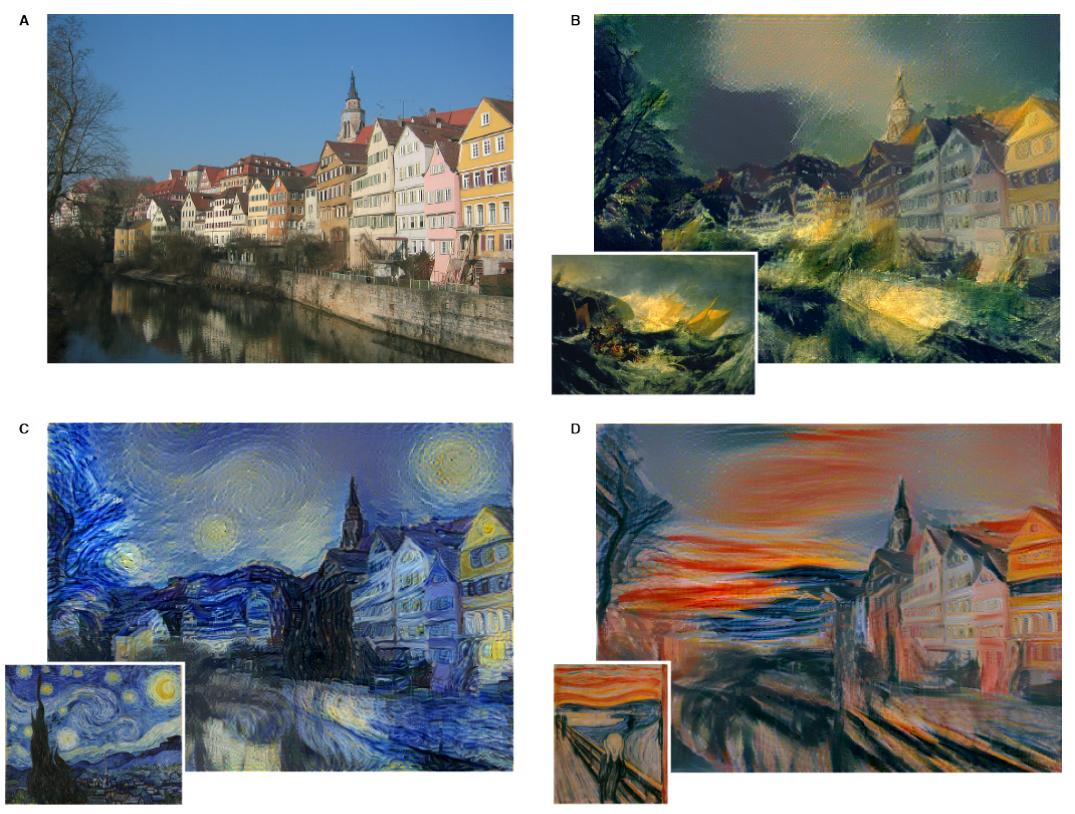
\includegraphics[trim = 0mm 0mm 0mm 0mm, clip, width=8.4cm]{style.PNG}
			\label{fig:res4}
		\end{figure}
\end{frame}

\begin{frame}{Recent Highlights}
		\begin{figure}
	  		\vspace*{0.1cm}
			\centering
			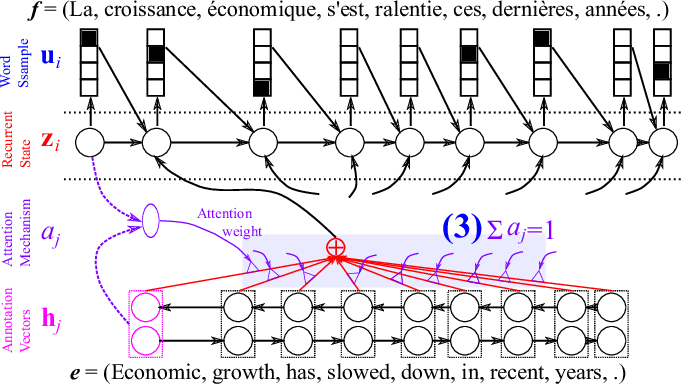
\includegraphics[trim = 0mm 0mm 0mm 0mm, clip, width=9.0cm]{machinetranslation.png}
			\label{fig:res4}
		\end{figure}
\end{frame}

\begin{frame}{Recent Highlights}
		\begin{figure}
	  		\vspace*{0.1cm}
			\centering
			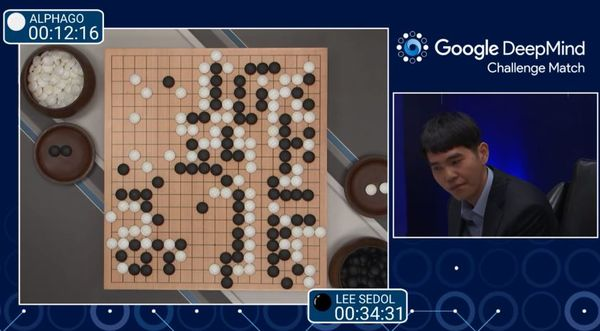
\includegraphics[trim = 0mm 0mm 0mm 0mm, clip, width=9.0cm]{alphago.jpg}
			\label{fig:res4}
		\end{figure}
\end{frame}

\begin{frame}{Recent Highlights}
		\begin{figure}
	  		\vspace*{-0.4cm}
	  		\hspace*{-0.5cm}
			\centering
			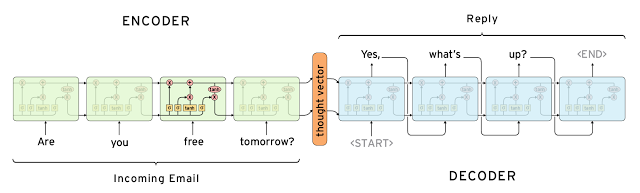
\includegraphics[trim = 0mm 0mm 0mm 0mm, clip, width=11.5cm]{chatbot1.png}
			\label{fig:res4}
		\end{figure}
				\begin{figure}
	  		\vspace*{-0.1cm}
			\centering
			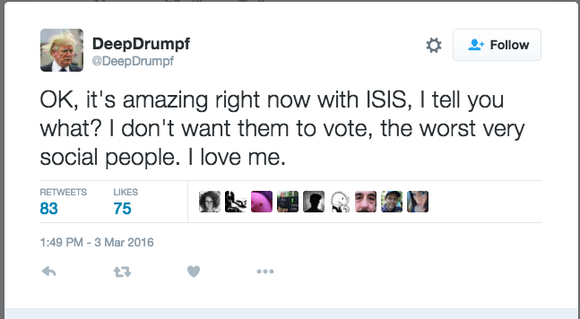
\includegraphics[trim = 5mm 5mm 5mm 5mm, clip, width=7.4cm]{chatbot3.png}
			\label{fig:res4}
		\end{figure}
\end{frame}

\begin{frame}{Other Examples}
\begin{itemize}
\item{Speech Recognition} \pause
\item{Decision Support Systems in Healthcare} \pause
\item{Predicting Epidemics From Social Media} \pause
\item{Targeted Advertising} \pause
\item{Anonymization \& Leveraging Security} \pause
\item{De-anonymization, Fraud Detection, Criminal Identification} \pause
\item{...} 
\end{itemize}
\end{frame}

\section{But, How Do These Work?}
\subsection{Teach Me Master}
\begin{frame}{But, How Do These Work?}
  		\begin{block}{(Most) Machine learning algorithms learn from examples, i.e., supervised learning.}
  		\end{block}
			 \pause
\vspace{0.3cm}
  		\begin{block}{Accuracies tend to increase with more data.}	
		\end{block} \pause
		\begin{center} \textbf{ \Large{
  		YOU ARE THE TEACHER!
  		} }
	\end{center}	
\end{frame}

\begin{frame}{But, How Do These Work?}
		\begin{figure}
	  		\vspace*{0.0cm}
			\centering
			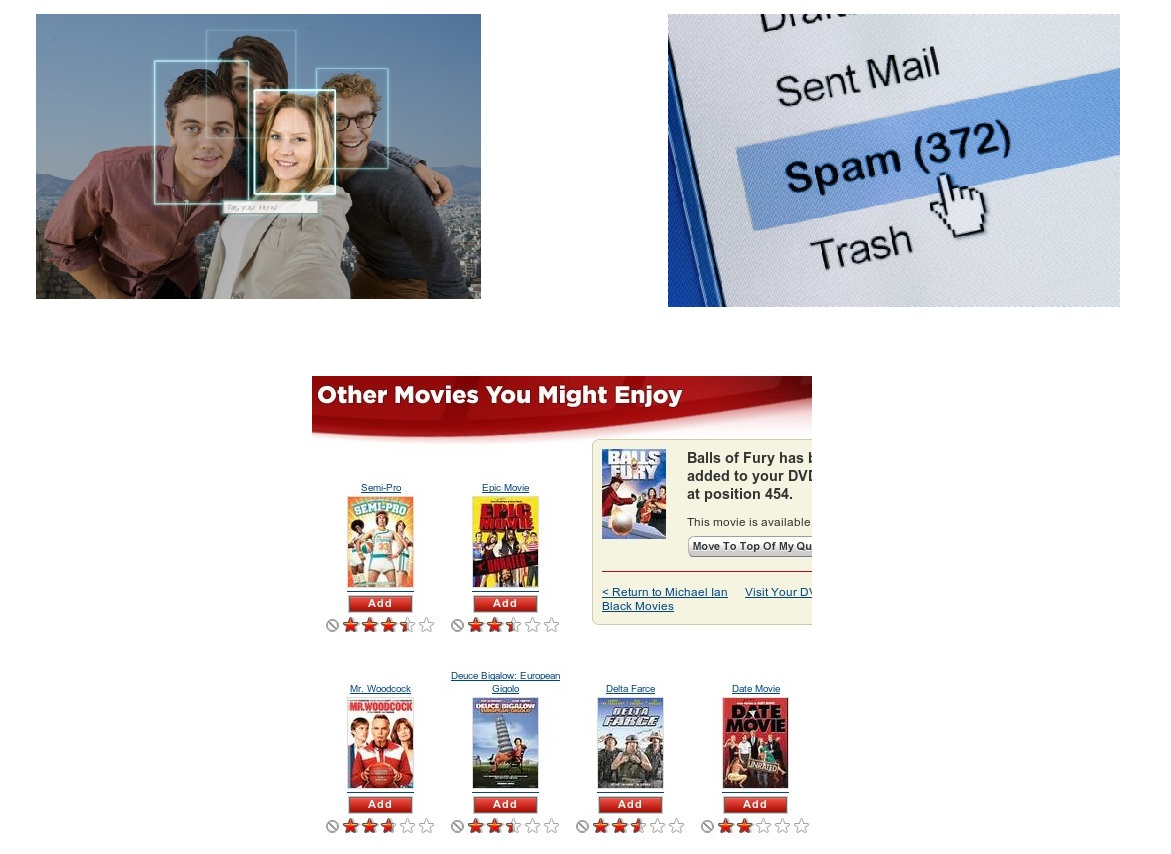
\includegraphics[trim = 0mm 0mm 0mm 0mm, clip, width=9.2cm]{fbface.jpg}
			\label{fig:res4}
		\end{figure}
\end{frame}
\subsection{There Is No Free Lunch!}
\begin{frame}{No Free Lunch Theorem}
\begin{block}{There is always a trade-off} \pause
\begin{itemize}
\item{Complexity \textbf{vs.} Interpretability \& Transparency}  \pause
\vspace{0.5cm}
\item{Accuracy \textbf{vs.} Computation Power}  \pause
\vspace{0.5cm}
\item{Specificity \textbf{vs.} Sensitivity} \pause
\vspace{0.5cm}
\item{Bias \textbf{vs.} Variance} \pause
\vspace{0.5cm}
\item{...} 
\end{itemize}
\end{block}
\end{frame}

\subsection{Inevitable Nature of Things}
\begin{frame}{An Example}
Certain patterns occur frequently in nature. \pause 
 \begin{block}{
 Normal (Gaussian) Distribution}
\end{block} \pause
		\begin{figure}
	  		\vspace*{0.1cm}
			\centering
			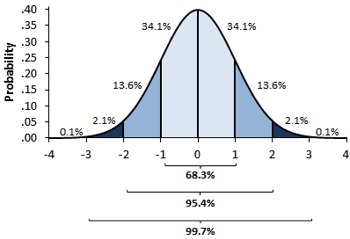
\includegraphics[trim = 0mm 0mm 0mm 0mm, clip, width=8.2cm]{normal.jpg}
			\label{fig:res4}
		\end{figure}
\end{frame}

\begin{frame}{Normal Distribution}
\begin{itemize}
\item{Velocity of Molecules in a Gas } \pause
\item{Human Height\footnote{Huxley, Julian S. (1932). Problems of Relative Growth.}} \pause
\item{Monthly Rainfall\footnote{Oosterbaan, Roland J. (1994). "Chapter 6: Frequency and Regression Analysis of Hydrologic Data". In Ritzema, Henk P. Drainage Principles and Applications}} \pause
\item{Stock Return Volatility\footnote{Andersen, Torben G., et al. (2001) "The distribution of realized stock return volatility." Journal of financial economics 61.1}} \pause
\end{itemize}
 \begin{block}{Why? $\Longrightarrow$ Central Limit Theorem}
\end{block}
\end{frame}

\begin{frame}{Inevitable Nature of Things}
		\begin{figure}
	  		\vspace*{-0.1cm}
			\centering
			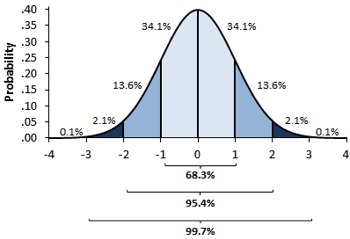
\includegraphics[trim = 0mm 10mm 0mm 0mm, clip, width=8.4cm]{normal.jpg}
			\label{fig:res4}
		\end{figure}
\begin{center}
There will be outliers, anomalies and under-represented groups/subsets!
\end{center}
\end{frame}

\subsection{Consequences}
\begin{frame}{Consequences}
\begin{center}
\textbf{\LARGE{
Supervised Algorithms \\ \pause + \\  Biased Data \\ \pause = \\ \vspace{0.4cm} Biased Algorithms}}
\end{center}
\end{frame}

\begin{frame}{Ugly Results}
If the training data reflect existing social biases against a minority, the algorithm is likely to incorporate these biases. \pause
\begin{block}{ }
Google's algorithms showing prestigious job ads to men, but not to women.\footnote{http://www.independent.co.uk/life-style/gadgets-and-tech/news/googles-algorithm-shows-prestigious-job-ads-to-men-but-not-to-women-10372166.html}
\end{block} \pause
\begin{block}{ }
Google image search in USA for \textit{``CEO''} produced 11 \% women, even though 27 \% of United States chief executives are women.\footnote{http://www.huffingtonpost.com/2015/04/10/google-image-gender-bias\_n\_7036414.html}
\end{block}
\end{frame}

\begin{frame}{Ugly Results}
Consider a loan application from a bank. Numerous attributes can be an input to a ML algorithm:
\begin{itemize}
\item{Age} 
\item{Field of Work} 
\item{Income} 
\item{Gender} 
\item{Marital Status}
\item{Residence District}
\item{Number of Children} 
\item{Transaction History} 
\item{Race}
\item{...} 
\end{itemize}
\end{frame}

\begin{frame}{Ugly Results}
Consider a loan application from a bank. Numerous attributes can be an input to a ML algorithm:
\begin{itemize}
\item{Age} 
\item{Field of Work} 
\item{Income} 
{\color{red}\item{Gender !} }
\item{Marital Status}
\item{Residence District}
\item{Number of Children} 
\item{Transaction History} 
{\color{red}\item{Race !}}
\item{...} 
\end{itemize}
\end{frame}

\begin{frame}{Ugly Results}
Anything else? \pause 
\begin{itemize}
\item{Age} 
\item{Field of Work} 
\item{Income} 
{\color{red}\item{Gender !} }
\item{Marital Status}
{\color{red}\item{Residence District !} }
\item{Number of Children} 
\item{Transaction History} 
{\color{red}\item{Race !}}
\item{...} 
\end{itemize}
\begin{block}{ }
Biases can be transferred through correlated attributes!
\end{block}
\end{frame}

\section{What Can Be Done?}

\subsection{Discrimination and Privacy-aware ML}
\begin{frame}{Discrimination and Privacy-aware ML}
Bias-free machine learning research should be encouraged.
\end{frame}

\subsection{Increased Transparency}
\begin{frame}{Transparent Design}
\begin{block}{ }
Is the decision explainable enough?
\end{block} \pause
\begin{block}{ }
Which attributes (features) have been used?
\end{block} \pause
\begin{block}{ }
Importance of attributes inferred by the algorithm?
\end{block}
\end{frame}

\begin{frame}{Transparent Reporting}
\begin{block}{ }
New ML algorithm predicts whether one has lung cancer or not with 90\% accuracy.
\end{block} \pause
\vspace{0.2cm}
\textbf{Overall accuracy is not enough. \\ \pause
\vspace{0.2cm}
Accuracies on different subgroups, false positive \& true negative rates.}
\end{frame}

\section{Where Are We Heading?}
\begin{frame}{Box Is Getting Blacker}
\begin{block}{ }
Black-box models (e.g. neural networks) are extremely popular!
\end{block}
\begin{block}{ }
\textit{``If it works, I don't care why!''} approach.
\end{block}
\end{frame}

\section*{Conclusion}
\begin{frame}{Conclusion}
\begin{block}{MyData is important:}
The fuel of ML algorithms! \pause
\end{block}
\begin{block}{Increased awareness on interaction of MyData \& algorithmic decision making systems is important:}
Promotes openness, transparency and bias-free ML approaches! 
 \end{block} 
\end{frame}

\begin{frame}{}
		\begin{figure}
	  		\vspace*{-0.0cm}
			\centering
			
\includegraphics[trim = 0mm 10mm 0mm 0mm, clip, width=10.4cm]{thanks.jpg}
			\label{fig:res4}
		\end{figure}
\end{frame}

\end{document}


